\chapter{Results}\label{ch:res}

\begin{flushright}{\slshape
    If it's not on fire, it's a software problem.\\ \medskip
    --- Unknown}
\end{flushright}

When designing a system aimed for performance, one has to test the system and
compare it to other solutions to see whether we have gained any mentionable
speedup.

As the assignment was to create an array-based
image processor, it is interesting to see how our system performs
at typical image processing tasks, and whether utilizing the \ac{SIMD}
array yields any performance advantages over doing everything in the
control core.

%As the assignment was to create an array-based image processor, it
%would be interesting to see how much more efficient our design is, depending on
%the amount of cores the system has.

In this chapter, we will present the results of our benchmarks of two
critical parts of the system; the SD card read performance of the
\ac{SCU} and the image processing performance of LENA. We will also show
screen shots from the system running several different image processing
programs.

%The first section will go into detail on the performance aspect of the results. We
%will here look at throughput, total processing time and other aspects related to
%performance, and compare them based on the number of cores we use. In the
%following section, we will have a look at the power consumption. We will measure
%how much power the system requires running with different cores, and how much
%power the system requires to process a single task with different amount of
%cores.

\section{SD Card Performance}
\label{sec:performance-sd-card}

As mentioned in section \ref{sec:avr-spi-issues}, reading data from an
SD card over SPI turned out to be the biggest bottleneck for throughput
in our system. In this section, we will document the optimizations we
made to improve the SD card's read performance.

Table \ref{tab:spi-optimizations-table} shows the gradually improving
performance as we optimized the code. This is also shown in figure
\ref{fig:spi-optimizations-plot}. Each of the optimizations are
explained in greater detail below.

\begin{description}
	\item[Removed status checking + function inlining] \hfill \\
		The spi\_send function busy-waited on the TXEMPTY flag for each
		byte it transmitted. In our case of alternating sends and reads,
		we do not have to check whether the SPI send register is empty
		every time. Inlining spi\_read and spi\_write also helped,
		although -O1, -O2 or -O3 would have done this for us.
	\item[Less SPI status register polling] \hfill \\
		In spi\_read, two conditions are busy-waited on before
		returning: whether the send register is empty, and whether the
		receive buffer is full yet. We only have to check the latter of
		these conditions.
	\item[Increased clock rate] \hfill \\
		Our CPU and main bus is driven by an external 12MHz crystal
		oscillator and the SPI clock frequency is calculated by dividing
		this by an integer number. We kept this divisor to be either 1
		or 2 (so SPI ran at either the same or half the speed of the
		CPU). Increasing to clock rate from 12MHz to 78 MHz boosted the
		speed from 157kB/s to 456 kB/s.
	\item[Compiler optimizations] \hfill \\
		Turning on compiler optimizations improved increase performance
		by another 14\%. There was no noticeable difference in
		performance from -O1, -O2 or -O3. However, compiler
		optimizations had a more profound effect on the overall system
		performance. We did not benchmark this extensively, but it was
		probably caused by optimizations the compiler made to the \ac{LENA}
		communication code.
	\item[Bypass FAT and use multiple block reads] \hfill \\
		We patched the framework code to support multiple block reads.
		Apparently, this was not something the FAT driver was able to
		take full advantage of out of the box. It was easier to simply
		bypass the file system than to try to fix it, so that is what we
		did.
		
		By reading the blocks directly from the SD card, we could read
		all 150 blocks of a picture in one function call. Limiting the
		file system to the first half of the SD card and add metadata
		files containing the block offsets into the second half of the
		card was easy. This more than doubled our performance, from 515
		kB/s to 1172 kB/s.
\end{description}

\TODO{This must be rewritten}
After implementing these optimizations, the \ac{SCU} was capable of pushing out around
12 FPS to the \ac{LENA}, around 920 kB/s. As we managed to reach our goal of 10
FPS, we did not optimize it any further. However, using the \ac{PDCA}, we could
have effectively eliminated the 25\% time spent sending to the \ac{LENA} while
the \ac{SD} card waited. Thus, giving as a frame rate of around 16
FPS. 
\begin{table}[H]
  \centering
  \begin{tabularx}{\textwidth}{c X r} \toprule
    \thx{Milestone} & \thx{Description} & \thx{Performance} \\
    \midrule
    1 & Baseline before optimization & 74.87 kB/s \\
    2 & Less status checking in {\tt spi\_send} plus inlining & 137.00 kB/s \\
    3 & Less \ac{SPI} status register polling & 156.59 kB/s \\
    4 & Clock rate of 20MHz, 10MHz \ac{SPI} & 214.40 kB/s \\
    5 & Clock rate of 20MHz, 20MHz \ac{SPI} & 243.00 kB/s \\
    6 & Clock rate of 40MHz, 20MHz \ac{SPI} & 327.80 kB/s \\
    7 & Clock rate of 48MHz, 24MHz \ac{SPI} & 369.50 kB/s \\
    8 & Clock rate of 60MHz, 30MHz \ac{SPI} & 423.40 kB/s \\
    9 & Clock rate of 72MHz, 36MHz \ac{SPI} & 432.70 kB/s \\
    10 & Clock rate of 78MHz, 39MHz \ac{SPI} & 455.80 kB/s \\
    11 & Turn on {\tt -O1} & 521.70 kB/s \\
    12 & Turn on {\tt -O2} & 523.40 kB/s \\
    13 & Turn on {\tt -O3} & 515.30 kB/s \\
    14 & Bypass \ac{FAT} and use multiple block reads & 1171.90 kB/s \\ 
    \bottomrule
  \end{tabularx}
  \caption[SPI Read Performance]{The read performance over \ac{SPI} at various
    milestones.}
  \label{tab:spi-optimizations-table}
\end{table}

\begin{figure}[H]
  \centering
  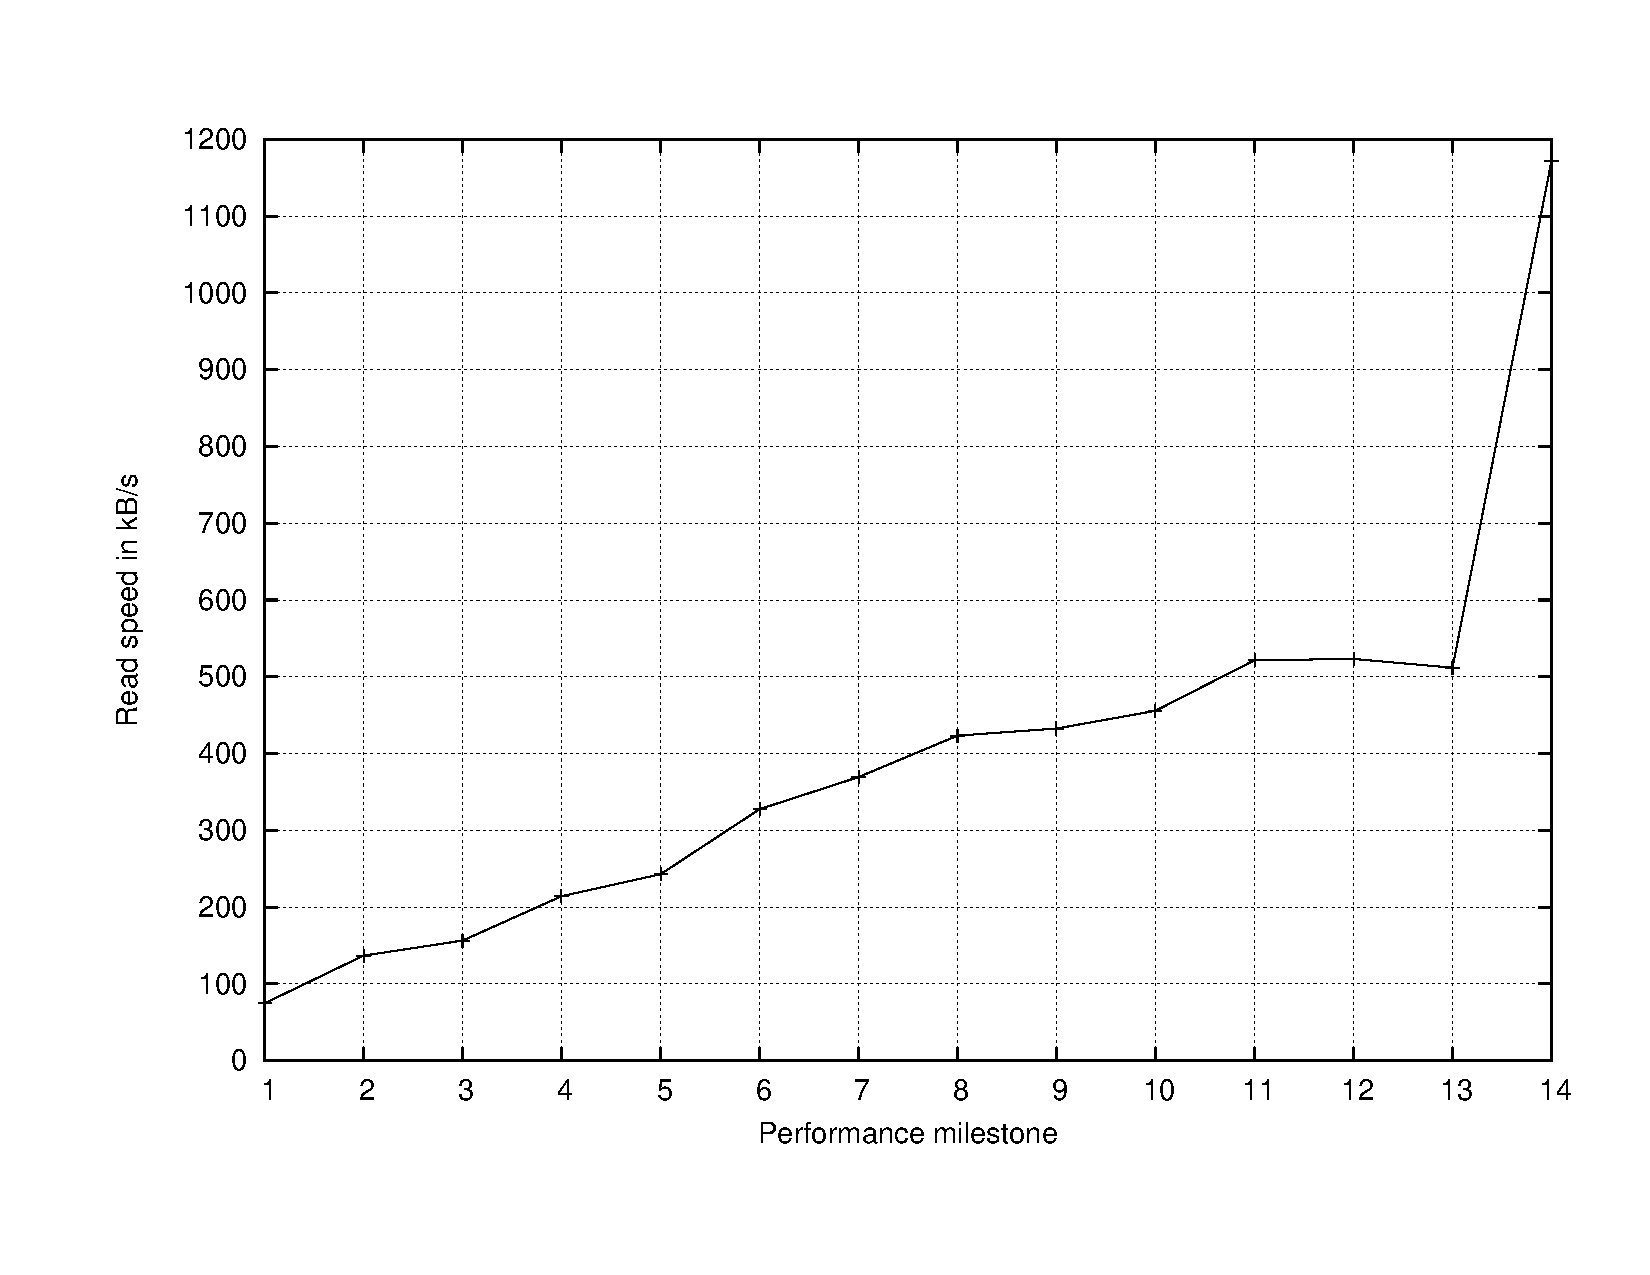
\includegraphics[width=\textwidth]{fig/avr/spi-optimizations-plot.pdf}
  \caption[SPI Optimizations Plot]{The results from Table
    \ref{tab:spi-optimizations-table} plotted. Milestones are along the
    $x$-axis and read performance along the $y$-axis.}
  \label{fig:spi-optimizations-plot}
\end{figure}


\chapter{LENA}

\section{SIMD Instruction Set}\label{apx:simd-instruction-set}

SIMD nodes operates on a {\tt 24 bit} instruction set divided in 2 main
formats. Arithmetic instructions (R, I and S) and message passing instructions
(M-send, M-store and M-forward).

\subsection[R Format]{R Format (OP = 000)}
Arithmetic register functions instructions

\begin{table}[h]
  \centering
  \begin{tabular}{cccccccc}\toprule
    \thx{ctrl} & \thx{mask} & \thx{op} & \thx{rs} & \thx{rt} & \thx{rd} &
    \thx{n/a} & \thx{fn} \\ \midrule
    1 bit & 1 bit & 3 bit & 4 bit & 4 bit & 4 bit & 4 bit & 3 bit
    \\ \bottomrule
  \end{tabular}
  \caption{Arithmetic register function instructions}
  \label{tab:ar-re-fu-in}
\end{table}


\begin{itemize}
\item {\tt ctrl} must be set to 0 in order to be executed on the SIMD node.
\item {\tt mask} is set to 1 to selectively enable the node when executing
  conditional branches.
\item {\tt op} the instruction opcode.
\item {\tt rs} write data register address.
\item {\tt rt} read data 1 register address.
\item {\tt rd} read data 2 register address.
\item {\tt n/a} not assigned for R instructions.
\item {\tt fn} the artimetic operation to perform.
\end{itemize}

\begin{table}[h]\small
  \centering
  \begin{tabularx}{1.03\textwidth}{lccX}\toprule
    \thx{name} & \thx{fn} & \thx{assembly code} & \thx{binary representation}
    \\ \midrule
    \thx{add} & \tt 000 & \tt add \$rs, \$rt, \$rd &
    \tt 0 m 000 ssss tttt dddd ---- 000\\
    \thx{sub} & \tt 001 & \tt sub \$rs, \$rt, \$rd &
    \tt 0 m 000 ssss tttt dddd ---- 001\\
    \thx{slt} & \tt 010 & \tt slt \$rs, \$rt, \$rd &
    \tt 0 m 000 ssss tttt dddd ---- 010\\
    \thx{and} & \tt 011 & \tt and \$rs, \$rt, \$rd &
    \tt 0 m 000 ssss tttt dddd ---- 011\\
    \thx{or}  & \tt 100 & \tt or~ \$rs, \$rt, \$rd &
    \tt 0 m 000 ssss tttt dddd ---- 100\\
    \thx{eq}  & \tt 101 & \tt eq~ \$rs, \$rt, \$rd &
    \tt 0 m 000 ssss tttt dddd ---- 101\\
    \thx{sll} & \tt 110 & \tt sll \$rs, \$rt, \$rd &
    \tt 0 m 000 ssss tttt ---- ---- 110\\
    \thx{srl} & \tt 111 & \tt srl \$rs, \$rt, \$rd &
    \tt 0 m 000 ssss tttt ---- ---- 111\\ \bottomrule
  \end{tabularx}
  \caption{List of R-instructions}
  \label{tab:r-instructions}
\end{table}


\subsection[I Format]{I Format (OP = 001)}
Immediate functions using constants.

\begin{table}[h]
  \centering
  \begin{tabular}{ccccccc}\toprule
    \thx{ctrl} & \thx{mask} & \thx{op} & \thx{rs} & \thx{rt} & \thx{const} &
    \thx{fn} \\ \midrule
    1 bit & 1 bit & 3 bit & 4 bit & 4 bit & 8 bit & 3 bit
    \\ \bottomrule
  \end{tabular}
  \caption{Immediate functions using constants}
  \label{tab:immediate-fn-const}
\end{table}


\begin{itemize}
\item {\tt ctrl} must be set to 0 in order to be executed on the SIMD node.
\item {\tt mask} is set to 1 for selectively enabling the node when executing
  conditional branches.
\item {\tt op} the instruction opcode.
\item {\tt rs} write data register address.
\item {\tt rt} read data 1 register address.
\item {\tt const} constant value | immediate.
\item {\tt fn} the artimetic operation to perform.
\end{itemize}

\TODO{Is the font size ok?}
\begin{table}[h]\small
  \centering
  \begin{tabularx}{1.03\linewidth}{lccX}\toprule
    \thx{name} & \thx{fn} & \thx{assembly code} & \thx{binary representation}
    \\ \midrule
    \thx{add} & \tt 000 & \tt addi \$rs, \$rt, \$rd &
    \tt 0 m 001 ssss tttt cccccccc 000\\
    \thx{sub} & \tt 001 & \tt subi \$rs, \$rt, \$rd &
    \tt 0 m 001 ssss tttt cccccccc 001\\
    \thx{slt} & \tt 010 & \tt slti \$rs, \$rt, \$rd &
    \tt 0 m 001 ssss tttt cccccccc 010\\
    \thx{and} & \tt 011 & \tt andi \$rs, \$rt, \$rd &
    \tt 0 m 001 ssss tttt cccccccc 011\\
    \thx{or}  & \tt 100 & \tt ori~ \$rs, \$rt, \$rd &
    \tt 0 m 001 ssss tttt cccccccc 100\\
    \thx{eq}  & \tt 101 & \tt eqi~ \$rs, \$rt, \$rd &
    \tt 0 m 001 ssss tttt cccccccc 101\\
    \thx{sll} & \tt 110 & \tt slli \$rs, \$rt, \$rd &
    \tt 0 m 001 ssss tttt -------- 110\\
    \thx{srl} & \tt 111 & \tt srli \$rs, \$rt, \$rd &
    \tt 0 m 001 ssss tttt -------- 111\\ \bottomrule
  \end{tabularx}
  \caption{List of I-instructions}
  \label{tab:i-instructions}
\end{table}


\subsection[S Format]{S Format (OP = 010)}
Swap source data register with processed data and store new source data in
register.

\begin{table}[h]
  \centering
  \begin{tabular}{cccccccc}\toprule
    \thx{ctrl} & \thx{mask} & \thx{op} & \thx{rs} & \thx{rt} & \thx{rd} &
    \thx{n/a} & \thx{fn} \\ \midrule
    1 bit & 1 bit & 3 bit & 4 bit & 4 bit & 4 bit & 4 bit & 3 bit \\ \bottomrule
  \end{tabular}
  \caption{S-format instructions}
  \label{tab:s-fmt-instr}
\end{table}


\begin{itemize}
\item {\tt ctrl} must be set to 0 in order to be executed on the SIMD node.
\item {\tt mask} set to 1 for selectively enabling the node when executing
  conditional branches.
\item {\tt op} the instruction opcode.
\item {\tt rs} new source data register address.
\item {\tt rt} old source data register address.
\item {\tt rd} must be 000000.
\item {\tt n/a} not assigned for S instructions.
\item {\tt fn} must be 000.
\end{itemize}

\begin{table}[h]\small
  \centering
  \begin{tabularx}{\textwidth}{lccX}\toprule
    \thx{name} & \thx{fn} & \thx{assembly code} & \thx{binary representation}
    \\ \midrule
    \thx{swap} & \tt 000 & \tt swap \$rs, \$rt &
    \tt 0 m 001 ssss tttt 0000 ---- 111\\ \bottomrule
  \end{tabularx}
  \caption{List of S instructions}
  \label{tab:s-instructions}
\end{table}



\subsection[M Format]{M Format (OP = 100, 101, 110)}
Send, receive and forward data from and to neighbor nodes in all directions
(north, south, east and west).

\begin{table}[h]
  \centering
  \begin{tabular}{cccccccc}\toprule
    \thx{ctrl} & \thx{mask} & \thx{op} & \thx{n} & \thx{s} & \thx{e} &
    \thx{w} & \thx{n/a} \\ \midrule
    1 bit & 1 bit & 3 bit & 4 bit & 4 bit & 4 bit & 4 bit & 3 bit \\ \bottomrule
  \end{tabular}
  \caption{M format instructions}
  \label{tab:m-fmt-instr}
\end{table}


\begin{itemize}
\item {\tt ctrl} must be set to 0 in order to be executed on the SIMD node.
\item {\tt mask} set to 1 for selectively enabling the node when executing
  conditional branches.
\item {\tt op} the instruction opcode.
\item {\tt n} north data write or read register address.
\item {\tt s} south data write or read register address.
\item {\tt e} east data write or read register address.
\item {\tt w} west data write or read register address.
\item {\tt n/a} no ALU operations applicable.
\end{itemize}

\begin{table}[h]
  \begin{tabularx}{\textwidth}{lrcc}\toprule
    \thx{name} & \thx{OP} & \thx{assembly code}
    \\ \midrule
    \thx{send} & \tt 100 & \tt send~ \$r1, \$r2, \$r3, \$r4\\
    \thx{store} & \tt 101 & \tt store \$r1, \$r2, \$r3, \$r4\\
    \thx{store \& forward} & \tt 110 & \tt frwrd \$r1, \$r2, \$r3, \$r4
    \\ \bottomrule
  \end{tabularx}
  \begin{tabularx}{\textwidth}{lX}
    \thx{name} & \thx{binary representation} \\ \midrule
    \thx{send} & 
    \tt 0 m 100 nnnn ssss eeee wwww ---\\
    \thx{store} &
    \tt 0 m 101 nnnn ssss eeee wwww ---\\
    \thx{store \& forward} & 
    \tt 0 m 110 nnnn ssss eeee wwww ---\\ \bottomrule
  \end{tabularx}    
  \caption{List of M-instructions}
  \label{tab:m-instructions}
\end{table}


In Table \ref{tab:m-instructions} we see the different \TODO{Something's amiss
  here} \ldots. \thx{store \& forward} forwards according to the 4-way data
exchange patterns (N $\rightarrow$ E, E $\rightarrow$ S, S $\rightarrow$ W, W
$\rightarrow$ N).

M-instructions must be issued with mask bit set to 0 in order to get data from
all the nodes. Otherwise, one will only get proper data from the ones executing
within a conditional branch. \CHECK{Should this be in an appendix, or?}

%\section{Control Core Instruction Set}

\TODO{Fill in.}

\section{LENA SCU bus}
\label{app:lena-scu-bus}

The LENA has two types of pins connected to the SCU. There are 9 I/O pins and 29 input pins. The I/O pins are mostly used for the LENA to acknowledge transfers, but the 8 remaining pins can be used for the fallback solution of having LENA transfer data back to the SCU. The 29 input pins are used to set LENA's state, acknowledge LENA and as a 24 bit wide one-way data bus used to transfer data and instructions to the LENA. Table \ref{tab:outbus}, \ref{tab:inbus} and \ref{tab:statebus} shows the pin mapping of the buses.

\begin{table}[h]
  \centering
  \begin{tabular}{l l} \toprule
    \thx{Line} & \thx{Usage}\\ \midrule
	LENA\_IO\_00..07 & Data bus (LSB..MSB)\\
	LENA\_IO\_CTRL & Interrupt / Ack from LENA.\\
  \end{tabular}
  \caption{LENA out bus}
  \label{tab:outbus}
\end{table}

\begin{table}[h]
  \centering
  \begin{tabular}{l l} \toprule
    \thx{Line} & \thx{Usage}\\ \midrule
	LENA\_IN\_00..23 & Data bus (LSB..MSB)\\
	LENA\_IN\_24 & Data bus ready\\ \bottomrule
  \end{tabular}
  \caption{LENA in bus}
  \label{tab:inbus}
\end{table}

\begin{table}[h]
  \centering
  \begin{tabular}{l l} \toprule
    \thx{Line} & \thx{Usage}\\ \midrule
	LENA\_IN\_25 & Set LENA state\\
	LENA\_IN\_26 & State bus (least significant bit)\\
	LENA\_IN\_27 & State bus\\
	LENA\_IN\_28 & State bus (most significant bit)\\ \bottomrule
  \end{tabular}
  \caption{LENA state bus}
  \label{tab:statebus}
\end{table}



\clearpage
\section{Code implementations}\label{apx:edgedetect}

\begin{code}
  \usemintedstyle{soderberg}
  \inputminted[frame=single,linenos,%firstline=50,firstnumber=50,%lastline=92,
    fontsize=\small]{lena}{lst/apx/lena/simd_embossing.lena}
  \caption{Emboss code in SIMD.}
  \label{lst:embossing}
\end{code}



\section{LENA screen shots}

In this section we show screen shots from the system running several
different image processing algorithms. The image used for the examples
is shown in Figure \ref{fig:lenna_unprocessed}. This figure shows a
screen shot when the system runs a simple \emph{show image/video}
program.

Figure \ref{fig:lenna_negated} shows the image after it has had its
colors negated by a program. Figure \ref{fig:lenna_embossed} shows the
image after being run through an embossing algorithm. In Figure
\ref{fig:lenna_edge_detected}, the image has been run through an edge
detection filter.

The images in these examples have all been processed by the cores in the
SIMD array.

\begin{figure}[h]
  \centering
  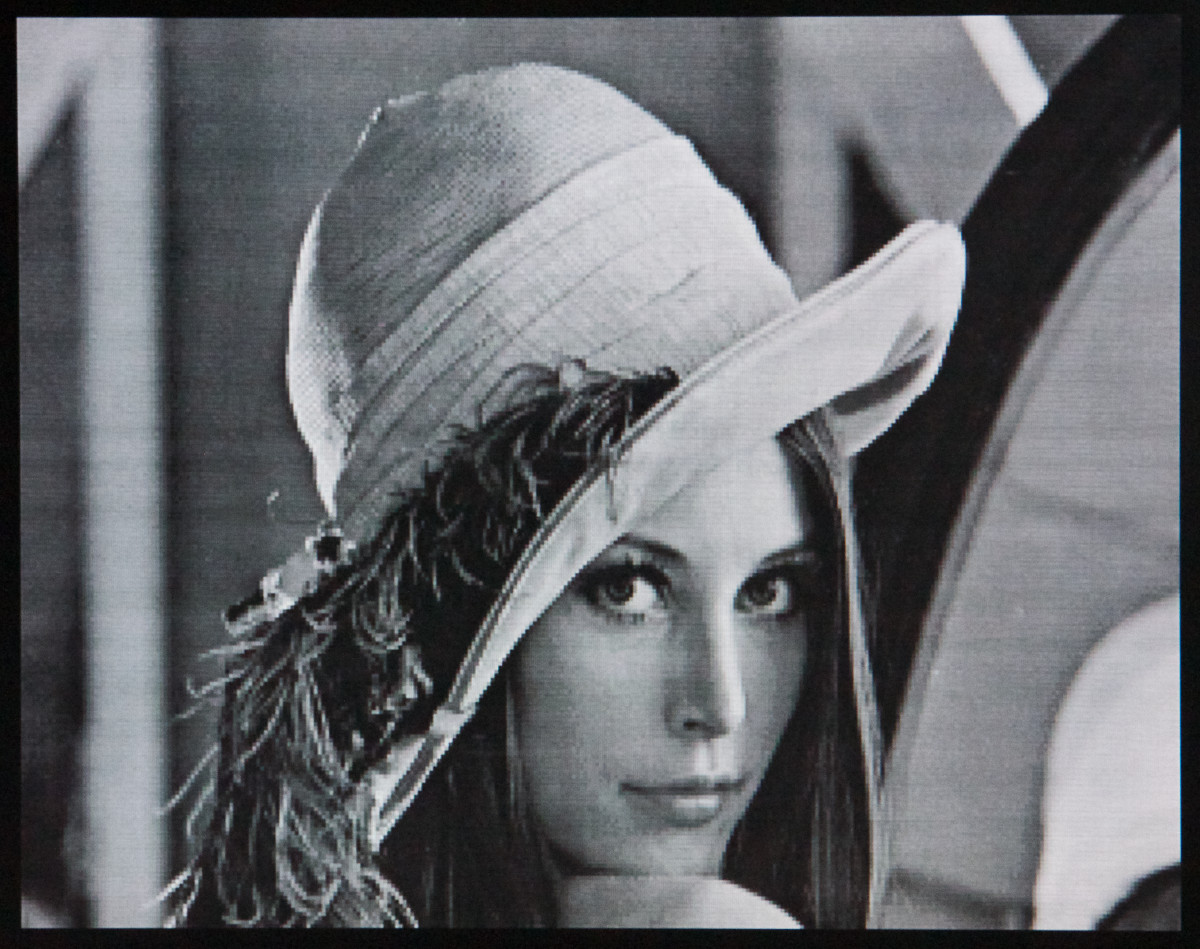
\includegraphics[width=0.8\textwidth]{gfx/results/lenna_unprocessed}
  \caption{Unprocessed image.}
  \label{fig:lenna_unprocessed}
\end{figure}

\begin{figure}[h]
  \centering
  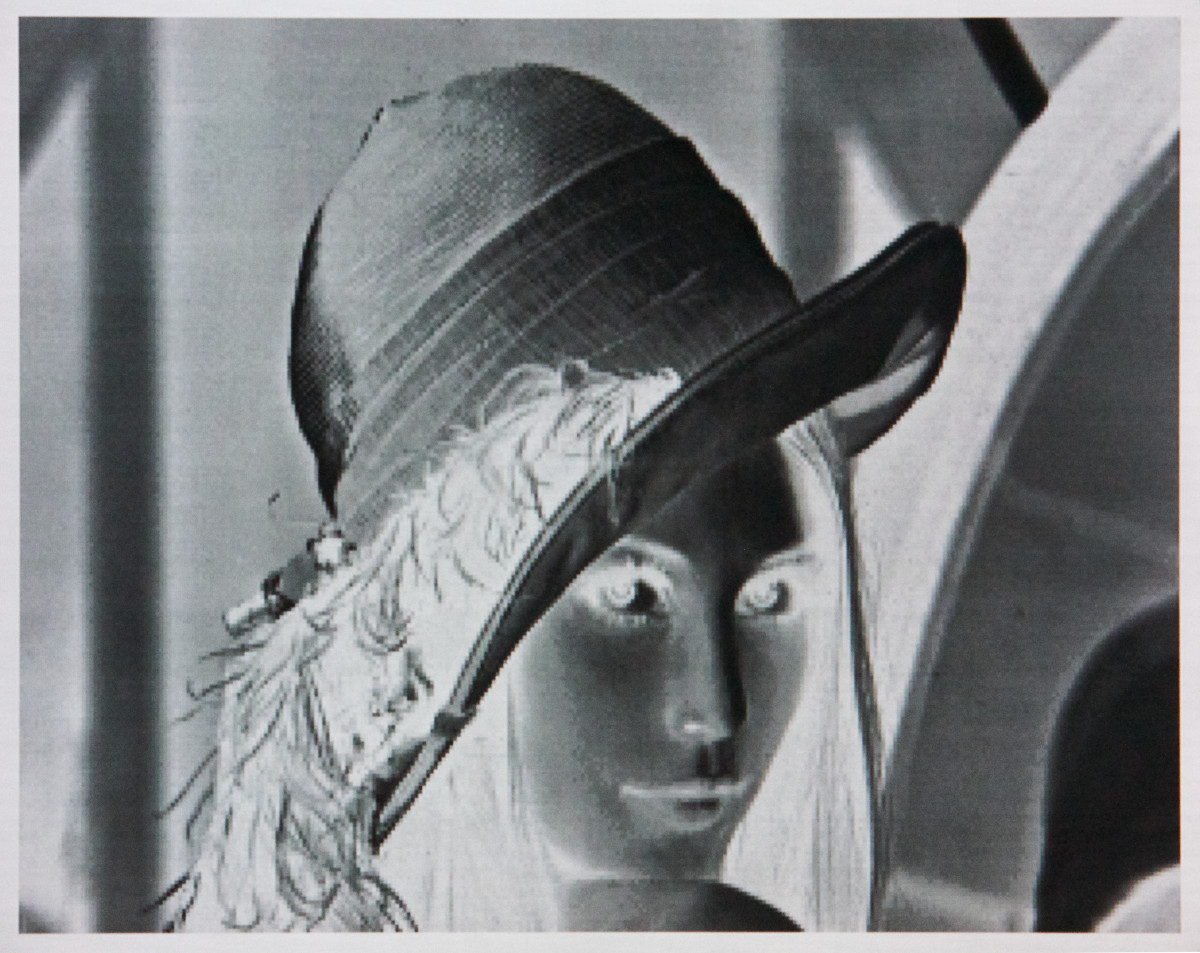
\includegraphics[width=0.8\textwidth]{gfx/results/lenna_negated}
  \caption{Negated image.}
  \label{fig:lenna_negated}
\end{figure}

\begin{figure}[h]
  \centering
  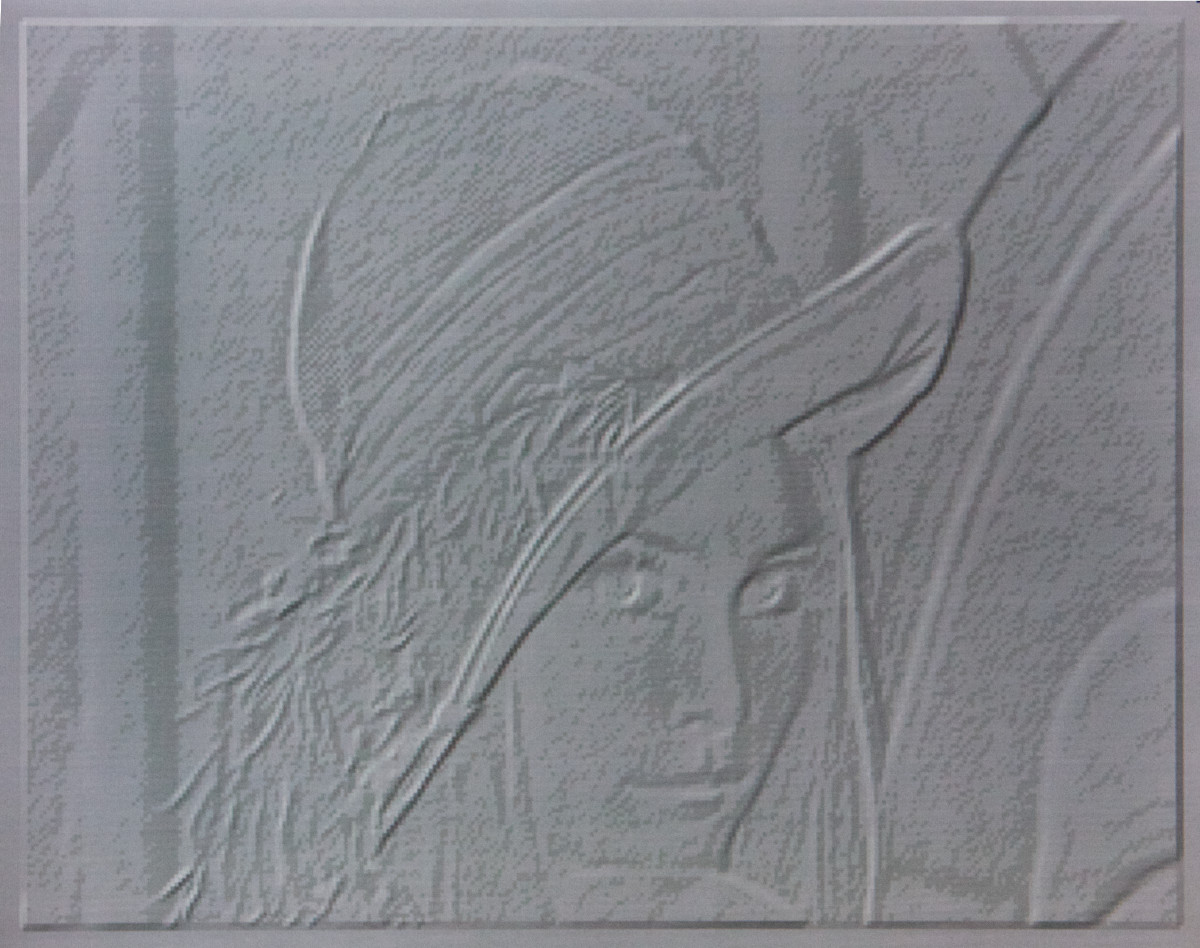
\includegraphics[width=0.8\textwidth]{gfx/results/lenna_embossed}
  \caption{Embossed image.}
  \label{fig:lenna_embossed}
\end{figure}

\begin{figure}[h]
  \centering
  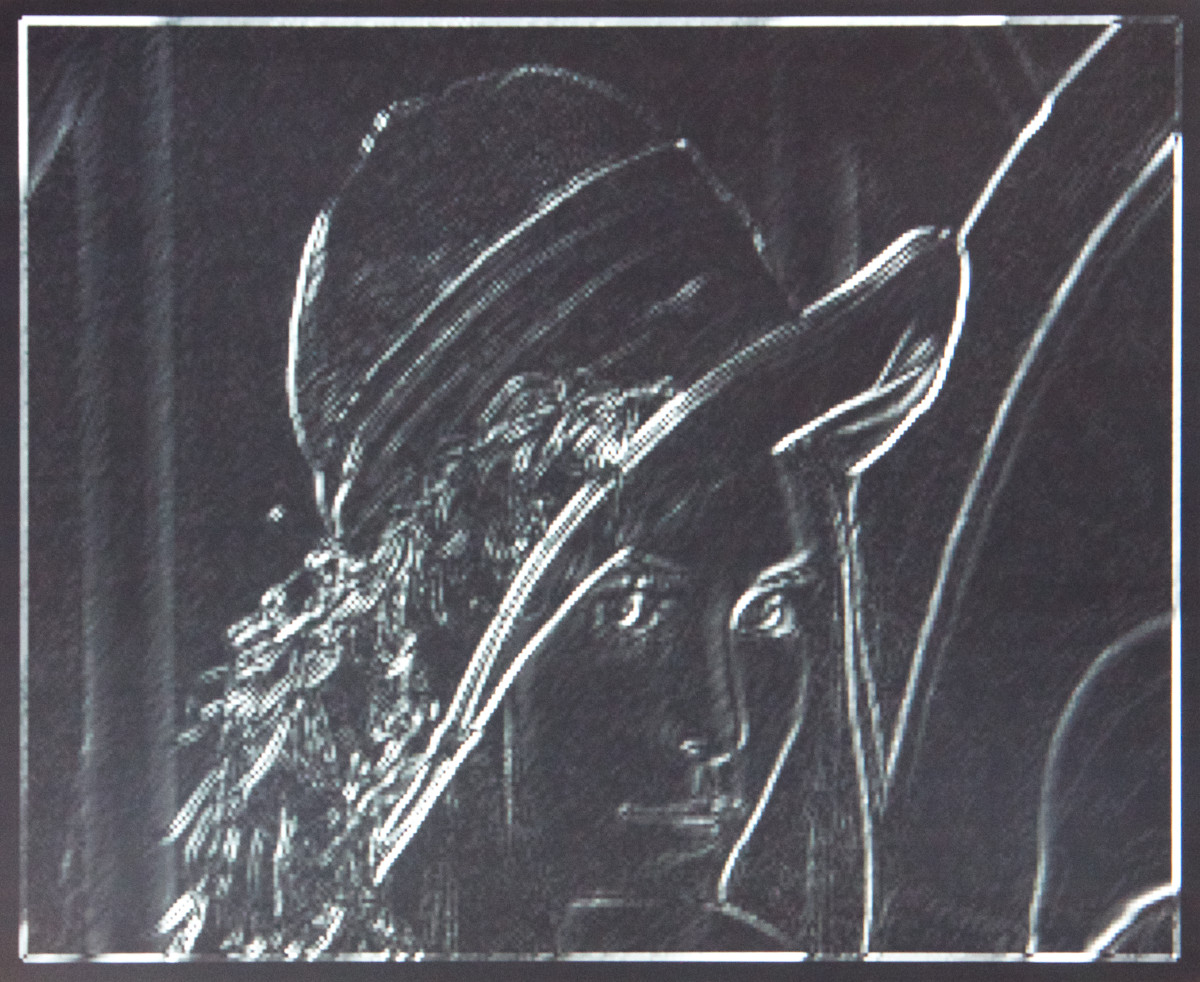
\includegraphics[width=0.8\textwidth]{gfx/results/lenna_edge_detected}
  \caption{Edge detected image.}
  \label{fig:lenna_edge_detected}
\end{figure}

